%%%%%%%%%%%%%%%%%%%%%%%%%%%%%%% beamer %%%%%%%%%%%%%%%%%%%%%%%%%%%%%%%%%%%%%%%%%%%%%%%%%
% To run - pdflatex filename.tex
%      acroread filename.pdf
%%%%%%%%%%%%%%%%%%%%%%%%%%%%%%%%%%%%%%%%%%%%%%%%%%%%%%%%%%%%%%%%%%%%%%%%%%%%%%%%%%%%%%%%

\documentclass[compress,oilve]{beamer}
\mode<presentation>

\usetheme[]{CambridgeUS}
% other themes: AnnArbor, Antibes, Bergen, Berkeley, Berlin, Boadilla, boxes, CambridgeUS, Copenhagen, Darmstadt, default, Dresden, Frankfurt, Goettingen,
% Hannover, Ilmenau, JuanLesPins, Luebeck, Madrid, Maloe, Marburg, Montpellier, PaloAlto, Pittsburg, Rochester, Singapore, Szeged, classic

\usecolortheme{beaver}
% color themes: albatross, beaver, beetle, crane, default, dolphin,  fly, lily, orchid, rose, seagull, seahorse, sidebartab, whale, wolverine

\usefonttheme{professionalfonts}
% font themes: default, professionalfonts, serif, structurebold, structureitalicserif, structuresmallcapsserif


\hypersetup{pdfpagemode=FullScreen} % makes your presentation go automatically to full screen

% define your own colors:
\definecolor{Red}{rgb}{1,0,0}
\definecolor{Blue}{rgb}{0,0,1}
\definecolor{Green}{rgb}{0,1,0}
\definecolor{magenta}{rgb}{1,0,.6}
\definecolor{lightblue}{rgb}{0,.5,1}
\definecolor{lightpurple}{rgb}{0.8, 0.6, 0.9}
\definecolor{gold}{rgb}{.6,.5,0}
\definecolor{orange}{rgb}{1,0.4,0}
\definecolor{hotpink}{rgb}{1,0,0.5}
\definecolor{newcolor2}{rgb}{.5,.3,.5}
\definecolor{newcolor}{rgb}{0,.3,1}
\definecolor{newcolor3}{rgb}{1,0,.35}
\definecolor{darkgreen1}{rgb}{0, .35, 0}
\definecolor{darkgreen}{rgb}{0, .6, 0}
\definecolor{darkred}{rgb}{.75,0,0}
\definecolor{skyblue}{HTML}{75bbfd}

\definecolor{olive}{cmyk}{0.64,0,0.95,0.4}
\definecolor{purpleish}{cmyk}{0.75,0.75,0,0}

% can also choose different themes for the "inside" and "outside"

% \usepackage{beamerinnertheme_______}
% inner themes include circles, default, inmargin, rectangles, rounded

% \usepackage{beamerouterthemesmoothbars}
% outer themes include default, infolines, miniframes, shadow, sidebar, smoothbars, smoothtree, split, tree


\useoutertheme[subsection=true, height=40pt]{smoothbars}

% to have the same footer on all slides
%\setbeamertemplate{footline}[text line]{STUFF HERE!}
\setbeamertemplate{footline}[text line]{} % makes the footer EMPTY
% include packages
%

%show the page numbers in footnote
%\addtobeamertemplate{navigation symbols}{}{%
	%	\usebeamerfont{footline}%
	%	\usebeamercolor[fg]{footline}%
	%	\hspace{1em}%
	%	\insertframenumber/\inserttotalframenumber
	%}

\setbeamercolor{footline}{fg=purpleish}
\setbeamerfont{footline}{series=\bfseries}

%add color to curent subsection
\setbeamertemplate{section in head/foot}{\hfill\tikz\node[rectangle, fill=darkred, rounded corners=1pt,inner sep=1pt,] {\textcolor{white}{\insertsectionhead}};}
\setbeamertemplate{section in head/foot shaded}{\textcolor{darkred}{\hfill\insertsectionhead}}

% Remove bullet of subsections
\setbeamertemplate{headline}
{%
	\begin{beamercolorbox}{section in head/foot}
		\insertsectionnavigationhorizontal{\textwidth}{}{}
	\end{beamercolorbox}%
}


% modify headlline, specially headline size
\setbeamertemplate{headline}{%
	\leavevmode%
	\hbox{%
		\begin{beamercolorbox}[wd=\paperwidth,ht=3.5ex,dp=1.125ex]{palette quaternary}%
			\insertsectionnavigationhorizontal{\paperwidth}{}{\hskip0pt plus1filll}
		\end{beamercolorbox}%
	}
}

\setbeamertemplate{footline}{%
	\leavevmode%
	\hbox{\begin{beamercolorbox}[wd=.5\paperwidth,ht=2.5ex,dp=1.125ex,leftskip=.3cm plus1fill,rightskip=.3cm]{author in head/foot}%
			\usebeamerfont{author in head/foot}\insertshortauthor ~ \insertshortinstitute
		\end{beamercolorbox}%
		\begin{beamercolorbox}[wd=.5\paperwidth,ht=2.5ex,dp=1.125ex,leftskip=.3cm,rightskip=.3cm plus1fil]{title in head/foot}%
			\usebeamerfont{title in head/foot}\insertshorttitle\hfill\insertframenumber\,/\,\inserttotalframenumber
	\end{beamercolorbox}}%
	\vskip0pt%
}


%\setbeamertemplate{navigation symbols}{}

\title{Introduction to ML and Classical ML Models}
\author{ML Instruction Team, Fall 2022}
\institute[]{CE Department \newline  Sharif University of Technology \newline \newline}
\date[\today]{}
%\titlegraphic{\includegraphics[scale=.35]{example-image}}



%Write \usepackage{etex} just after the \documentclass line (it should be the first loaded package).
\usepackage{etex}
\usepackage{subcaption}
\usepackage{multicol}
\usepackage{amsmath}
\usepackage{epsfig}
\usepackage{graphicx}
\usepackage[all,knot]{xy}
\xyoption{arc}
\usepackage{url}
\usepackage{multimedia}
\usepackage{hyperref}
\hypersetup{colorlinks,linkcolor=blue,citecolor=redorange,urlcolor=darkred}
\usepackage{multirow}
\usepackage[font={scriptsize}]{caption}
\usepackage{pgf}
\usepackage{fontspec}
%\setsansfont[Scale=MatchLowercase, BoldFont = * Bold, ItalicFont = * Italic]{Caladea}

%\usepackage{enumitem,xcolor}
%\newcommand{\labelitemi}{$\blacksquare$}
%\newcommand{\labelitemii}{$\diamond$}
%\newcommand{\labelitemiii}{$\square$}
%\newcommand{\labelitemiv}{$\ast$}
%\setbeamercolor*{item}{fg=red}


\usefonttheme{professionalfonts} 
\setbeamertemplate{itemize item}{\color{skyblue}$\blacksquare$}
\setbeamertemplate{itemize subitem}{\color{hotpink}$\blacktriangleright$}
\setbeamertemplate{itemize subsubitem}{\color{orange}$\bullet$}


\usepackage{anyfontsize}
\usepackage{t1enc}
\usepackage{tikz}
\usetikzlibrary{calc,trees,positioning,arrows,chains,shapes.geometric,decorations.pathreplacing,decorations.pathmorphing,shapes,matrix,shapes.symbols}



\newtheorem{proposition}[theorem]{Proposition}
\newtheorem{remark}[theorem]{Remark}
\newtheorem{assumption}[theorem]{Assumption}

\usepackage{xcolor}
\newcommand{\tc}[2]{
	\textcolor{#1}{\hspace{-2pt}#2\hspace{-2pt}}
}

%\usepackage{fontspec, unicode-math}
%\setmainfont[Scale=0.9]{Nimbus Roman No9 L}
%\setmonofont[Scale=0.9]{Monaco}
\setsansfont[Scale=1]{Times New Roman}

\newcommand{\vect}[1]{\boldsymbol{#1}}

\definecolor{strings}{rgb}{.624,.251,.259}
\definecolor{keywords}{rgb}{.224,.451,.686}
\definecolor{comment}{rgb}{.322,.451,.322}


%\usepackage{smartdiagram}
%\usesmartdiagramlibrary{additions}
%%%%%%%%%%%%%%%%%%%%%%%%%%%%%%%%%%%%%%%%%%%%%%%%%%%%%%%%%%%%%%%%%%%%%%%%%%%%%%%%%%%%%%%%%%%%
%%%%%%%%%%%%%%%%%%%%%%%%%%%%%% Title Page Info %%%%%%%%%%%%%%%%%%%%%%%%%%%%%%%%%%%%%%%%%%%
%%%%%%%%%%%%%%%%%%%%%%%%%%%%%%%%%%%%%%%%%%%%%%%%%%%%%%%%%%%%%%%%%%%%%%%%%%%%%%%%%%%%%%%%%%


%%%%%%%%%%%%%%%%%%%%%%%%%%%%%%%%%%%%%%%%%%%%%%%%%%%%%%%%%%%%%%%%%%%%%%%%%%%%%%%%%%%%%%%%%%
%%%%%%%%%%%%%%%%%%%%%%%%%%%%%% Begin Your Document %%%%%%%%%%%%%%%%%%%%%%%%%%%%%%%%%%%%%%%
%%%%%%%%%%%%%%%%%%%%%%%%%%%%%%%%%%%%%%%%%%%%%%%%%%%%%%%%%%%%%%%%%%%%%%%%%%%%%%%%%%%%%%%%%%

\begin{document}
	
%%%%%%%%%%%%%%%%%%%%%%%%%%%%%%%%%%%%%%%%%%%%%%%%%%%%%%%%%%%%%%%%%%%%%%%%%%%%%%%%%%%%%%%%%%
	\fontsize{9}{9}
\begin{frame}[noframenumbering, plain]
	\titlepage
\end{frame}

%%%%%%%%%%%%%%%%%%%%%%%%%%%%%%%%%%%%%%%%%%%%%%%%%%%%%%%%%%%%%%%%%%%%%%%%%%%%%%%%%%%%%%%%%%
\section{Introduction}
%%%%%%%%%%%%%%%%%%%%%%%%%%%%%%%%%%%%%%%%%%%%%%%%%%%%%%%%%%%%%%%%%%%%%%%%######
\frame{\frametitle{Machine Learning: an Overview}
\begin{itemize}
	\item \textcolor{keywords} {What is Machine Learning?} \\
	\medskip

	Machine learning is the field of study that gives computers the ability to learn without being explicitly programmed. 
		
	\item \textcolor{keywords}{Applications of Machine Learning}
	\begin{itemize}
		\item \href{https://thispersondoesnotexist.com/}{This Person Does not Exist!}
		
		\medskip
		\item \href{https://github.com/features/copilot}{Github Copilot}
		
		\medskip
		\item \href{https://imagen.research.google/}{Imagen}
		
		\medskip
		\item \href{https://www.craiyon.com/}{Dall-E Open AI}
		
		\medskip
		\item \href{https://www.impira.com/product/docquery}{DocQuery}
		
		\medskip
		\item \href{https://huggingface.co/spaces/adirik/OWL-ViT}{Zero Shot Object Detection!}
	\end{itemize}	
	
\end{itemize}

}
%%%%%%%%%%%%%%%%%%%%%%%%%%%%%%%%%%%%%%%%%%%%%%%%%%%%%%%%%%%%%%%%%%%%%%%%%
\section{ML Variations}

%%%%%%%%%%%%%%%%%%%%%%%%%%%%%%%%%%%%%%%%%%%%%%%%%%%%%%%%%%%%%%%%%%%%%%%%%
\begin{frame}{Machine Learning Categories}

\begin{figure}
	\centering
	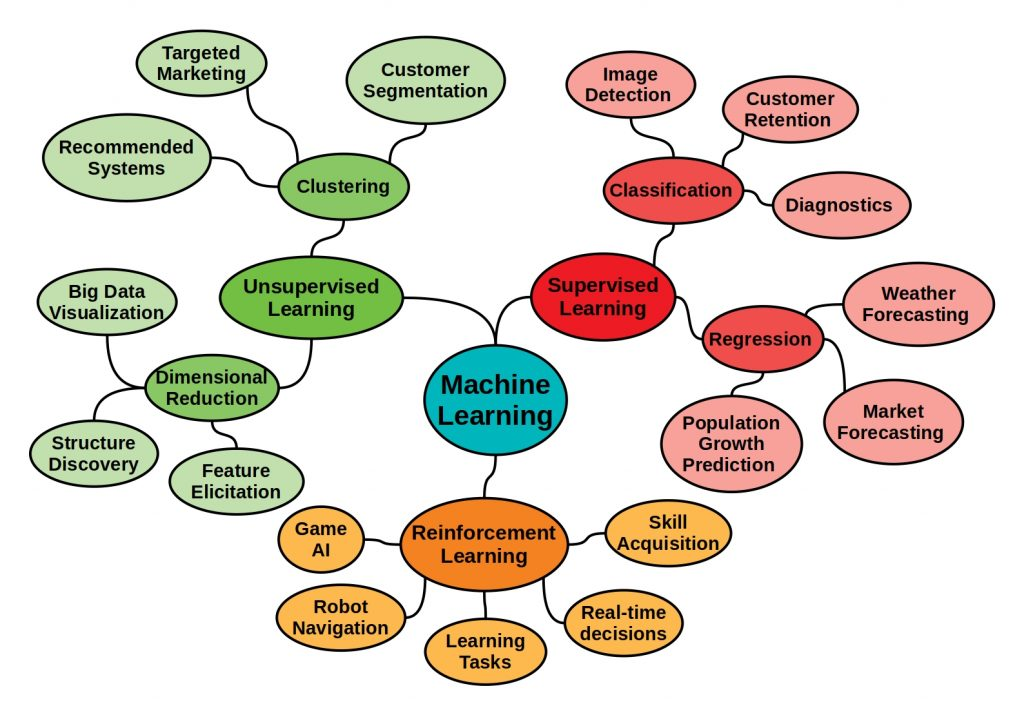
\includegraphics[scale=0.35]{Figs/1.jpeg}
	\caption{Classical Machine Learning Paradigm, \href{https://tinyurl.com/2zldw3my}{Source}}
\end{figure}
\end{frame}


%%%%%%%%%%%%%%%%%%%%%%%%%%%%%%%%%%%%%%%%%%%%%%%%%%%%%%%%%%%%%%%%%%%%%%%%%%
%%%%%%%%%%%%%%%%%%%%%%%%%%%%%%%%%%%%%%%%%%%%%%%%%%%%%%%%%%%%%%%%%%%%%%%%%%
\begin{frame}{Machine Learning Categories}
	\begin{itemize}
	\item The three broad categories of ML are summarized in:
		\begin{itemize}
		\item \textbf{Supervised Learning}
		\item \textbf{Unsupervised Learning}  
		\item \textbf{Reinforcement Learning} 
		\end{itemize}
	\end{itemize}
	\begin{figure}
		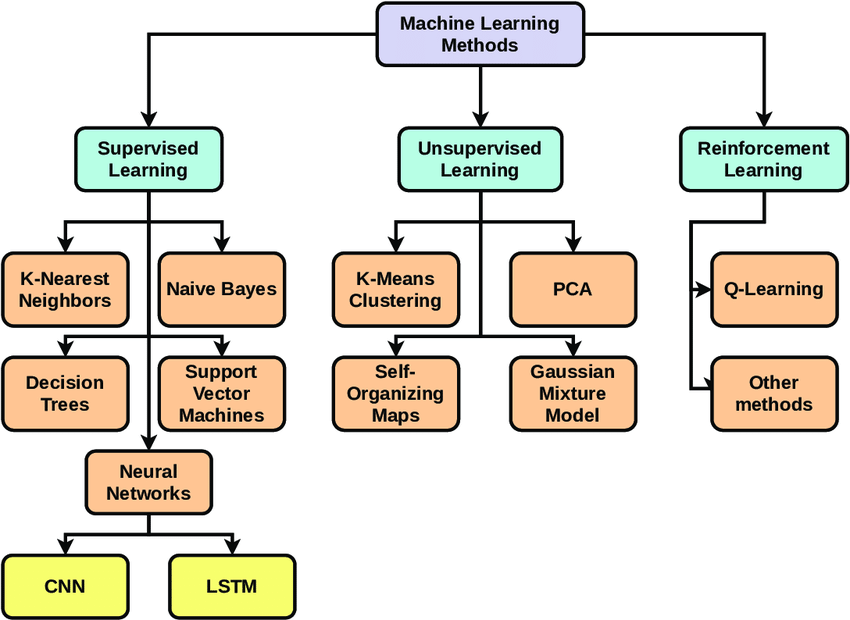
\includegraphics[width=8cm, height=5cm]{Figs/2-1.png}
		\caption{Categories of ML, \href{https://tinyurl.com/2qkt8vza}{Source}}
	\end{figure}
\end{frame}

%%%%%%%%%%%%%%%%%%%%%%%%%%%%%%%%%%%%%%%%%%%%%%%%%%%%%%%%%%%%%%%%%%%%%%%%%%

\begin{frame}{Supervised Learning}
	\begin{itemize}
		\item \tc{keywords}{Whats is Supervised Learning?}\\
		\medskip
		\tc{keywords}{Supervised Learning} is the subcategory of machine learning that focuses on learning from labeled training data, which can be divided to two main categories:
	
	\medskip
	\begin{itemize}
		\item \tc{keywords}{Classification}: Predicting the discrete values such as male/female, etc.
		\item \tc{keywords}{Regression}: Predicting the continuous values such as price, age, etc.
	\end{itemize}

	\end{itemize}

\begin{figure}[htbp!]
	\centering
	{
		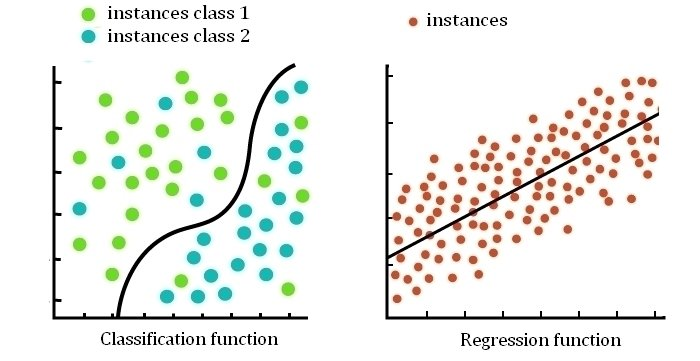
\includegraphics[width=8cm, height=4cm]{Figs/3.png}
	}
	\caption{Classification vs Regression, \href{https://tinyurl.com/2kvrm8jf}{Source}}
	\label{fig:globalfigure5}
\end{figure}


\end{frame}

%%%%%%%%%%%%%%%%%%%%%%%%%%%%%%%%%%%%%%%%%%%%%%%%%%%%%%%%%%%%%%%%%%%%%%%%%%

\begin{frame}{Unsupervised Learning}
	\begin{itemize}
	\item \tc{keywords}{What is Unsupervised Learning?}\\
	\medskip
	
	\tc{keywords}{Unsupervised Learning}, in contrast to supervised learning, is concerned with unlabeled data. 
	
	\medskip
	\item Common tasks in unsupervised learning are:
	
	\begin{itemize}
		\item \tc{keywords}{Clustering}  
		\item \tc{keywords}{Dimensionality Reduction}
	\end{itemize}
	
	\begin{figure}[htbp!]
		\subfloat[][Clsutering, \href{https://tinyurl.com/2m7cnlur}{Source}]
		{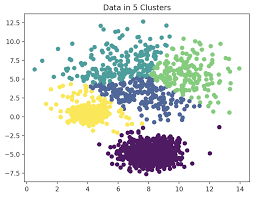
\includegraphics[width=4cm, height=3cm]{Figs/4.png}
			\label{fig:subfigure1}}
		\qquad
		\subfloat[][Dimensionality Reduction, \href{https://tinyurl.com/2z5gvlor}{Source}]
		{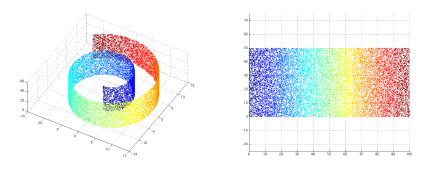
\includegraphics[width=6cm, height=3cm]{Figs/5.png}
			\label{fig:subfigure2}}
		\\
		
		\tiny
		\caption{Clustering vs Dimensionality Reduction}
		\label{fig:globalfigure2}
		
	\end{figure}
	
	\end{itemize}
\end{frame}
%%%%%%%%%%%%%%%%%%%%%%%%%%%%%%%%%%%%%%%%%%%%%%%%%%%%%%%%%%%%%%%%%%%%%%%%%%

\begin{frame}{Reinforcement Learning}
\begin{itemize}
	\item Reinforcement is the process of learning from rewards while performing a series of actions.
	
	\item An agent in this context is a learning system that observes the environment, selects and performs actions, and receives rewards. 
	
	\item As time goes on, it must learn how to get the most rewards using the best strategy, called a policy.
	
\end{itemize}

	\begin{figure}
		 \centering
		 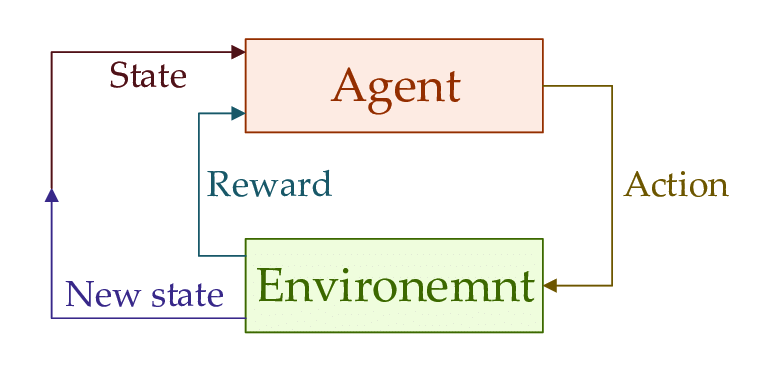
\includegraphics[width=6cm, height=3cm]{Figs/6.png}  
		 \caption{Reinforcement Learning, \href{https://tinyurl.com/2f6plway}{Source}.}
	\end{figure}

\end{frame}
%%%%%%%%%%%%%%%%%%%%%%%%%%%%%%%%%%%%%%%%%%%%%%%%%%%%%%%%%%%%%%%%%%%%%%%%%%
\begin{frame}{ML Categorization Schemes}
	\begin{itemize}
		\item Eager vs Lazy:
		\begin{itemize}
			\item \tc{keywords}{Eager} learners are algorithms that process training data immediately.
			
			\item \tc{keywords}{Lazy} learners, however, defer the processing step until the prediction. 
			
		\end{itemize}
	
	\medskip
		\item Batch vs Online:
		
		\begin{itemize}
			\item \tc{keywords}{Batch} learning refers to the fact that the model is learned on the entire set of training examples.
			
			\item \tc{keywords}{Online} learners, in contrast, learn from one training example at the time. 
			
		\end{itemize}
	
		\medskip
		\item Generative vs Discriminative:
		
				
		\begin{itemize}
			\item \tc{keywords}{Generative} models (classically) describe methods that
			model the joint distribution $\mathbb{P}(X, Y ) = \mathbb{P}(Y )\mathbb{P}(X|Y ) = \mathbb{P}(X)\mathbb{P}(Y|X)$ for training pairs $(x_i, y_i)$.
			
			
			\item \tc{keywords}{Discriminative} Discriminative models are taking a more "direct" approach, modeling $\mathbb{P}(Y|X)$ directly. 
			
		\end{itemize}
	\end{itemize}
\end{frame}
%%%%%%%%%%%%%%%%%%%%%%%%%%%%%%%%%%%%%%%%%%%%%%%%%%%%%%%%%%%%%%%%%%%%%%%%%%
\begin{frame}{ML Categorization Schemes}
	\begin{itemize}
		\item Instance-based vs Model-Based:
		\begin{itemize}
			\item \tc{keywords}{Instance-Based} learners learn the training examples by heart and then generalizes to new instances based on some similarity measure.
			
			\begin{itemize}
				\item Here, the algorithm looks at a set of training data and tries to find a pattern that can be generalized to new data.
				
				\item This pattern is then used to make predictions on new data.
			\end{itemize}
			
			\item \tc{keywords}{Model-Based} learners, on the other hand, learn from a model that is created from the training data.
			
			\begin{itemize}
				\item This model can be thought of as a mathematical representation of the training data.
				\item The model is then used to make predictions on new data.
			\end{itemize}
		\end{itemize}
		
		\medskip
		\item Parametric vs Non-parametric:
		
		\begin{itemize}
			\item \tc{keywords}{Parametric} models have "fixed" number of parameters.
			
			\item \tc{keywords}{Non-Parametric}
			models are more "flexible" and do not have a pre-specified number of parameters.
			
		\end{itemize}
		
		\medskip
	\end{itemize}
\end{frame}


%%%%%%%%%%%%%%%%%%%%%%%%%%%%%%%%%%%%%%%%%%%%%%%%%%%%%%%%%%%%%%%%%%%%%%
\section{ML in Practice}
%%%%%%%%%%%%%%%%%%%%%%%%%%%%%%%%%%%%%%%%%%%%%%%%%%%%%%%%%%%%%%%%%%%%%%%%%
\begin{frame}{How to Solve a Machine Learning Problem}
	\begin{itemize}
		\item Collect data.
		\item Preprocess the data.
		\item Select a suitable model and train it.
		\item Evaluate the generalization error on the test dataset.
		\item Improve the model using various techniques.
	\end{itemize}

	\begin{figure}
	 \centering
	 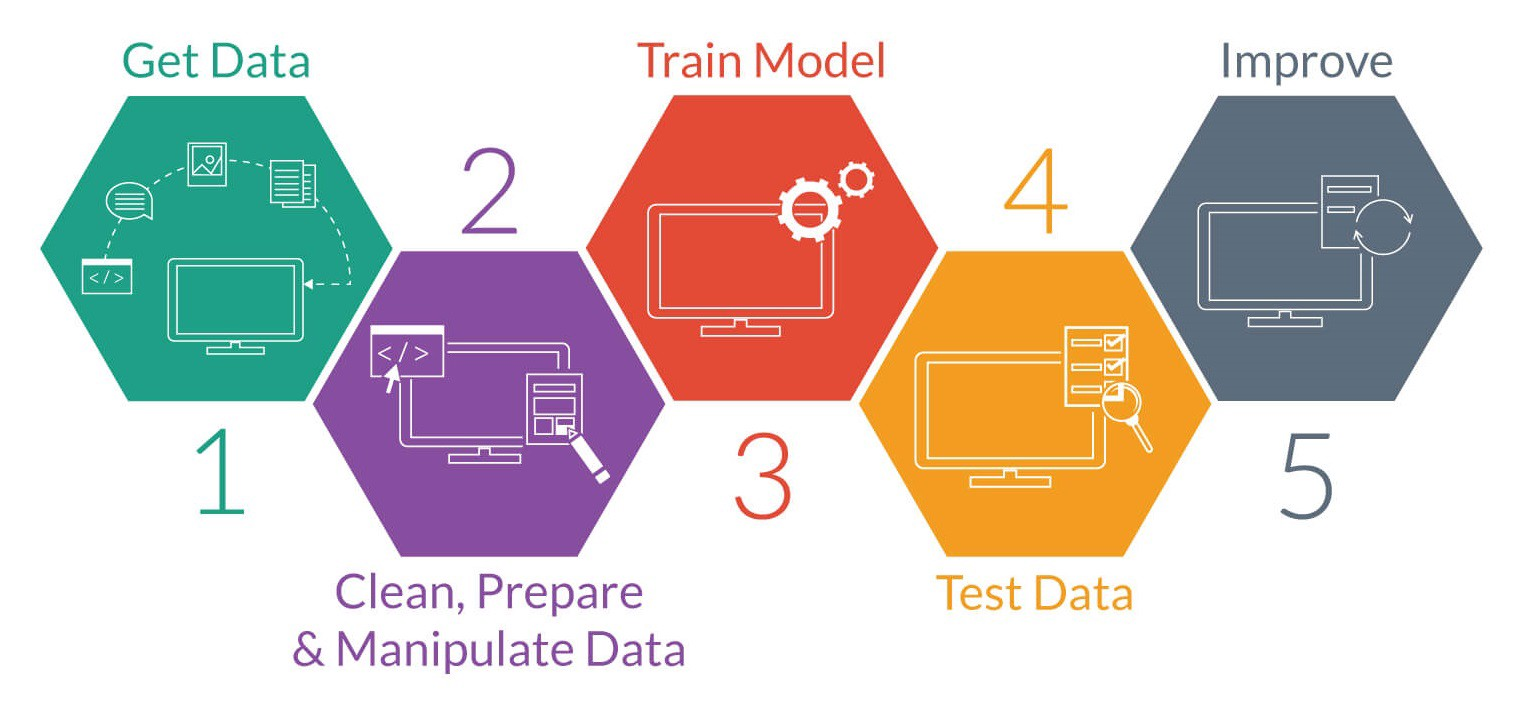
\includegraphics[width=6cm, height=3cm]{Figs/7.jpeg}  
	 \caption{Required steps to solve an ML problem, \href{https://tinyurl.com/2m7epjl2}{Source}}
	\end{figure}

\end{frame}

%%%%%%%%%%%%%%%%%%%%%%%%%%%%%%%%%%%%%%%%%%%%%%%%%%%%%%%%%%%%%%%%%%%%%%

\frametitle{Final Notes}
\centering
\vspace{50 pt}
\textbf{Thank You!}
\vspace{50pt}

\textbf{Any Question?}
%%%%%%%%%%%%%%%%%%%%%%%%%%%%%%%%%%%%%%%%%%
\end{document}